\documentclass[11pt, a4paper]{article}

\usepackage[T1]{fontenc}
\usepackage[utf8]{inputenc}
\usepackage{amsmath}
\usepackage{amssymb}
\usepackage{amsfonts}
\usepackage{amsthm}
\usepackage{bbm}
\usepackage{graphicx}
\usepackage{verbatim}
\usepackage{caption}
\usepackage{subcaption}
\usepackage{subfig}
\usepackage{float}

\newcommand{\vb}{\mathbf}


\renewcommand{\contentsname}{Innhald}
\renewcommand{\abstractname}{Samandrag}

\begin{document}

\begin{titlepage}

  \title{\normalsize FYS1120 Elektromagnetisme\\
    \vspace{10mm}
    \huge Labøving\\
    \vspace{10mm}
    \normalsize{\bf Grunnleggende elektromagnetisk måleteknikk.}}

  \author{Kristian Tuv, Hilde Solesvik Skeie og Øyvind Sigmundson Schøyen.}

\end{titlepage}

\maketitle

\newpage
  \tableofcontents
\newpage

\section*{Indre resistans i eit voltmeter}
\addcontentsline{toc}{section}{Indre resistans i eit voltmeter}

  \subsection*{Oppgåve 1.1}
  \addcontentsline{toc}{subsection}{Oppgåve 1.1}
    Me lader fort opp kondensatoren ved hjelp av batteriet. Me koplar deretter ut batteriet og koplar kondensatoren til voltmeteret.
    Programmet $\texttt{Oppgave1.1.py}$ plottar verdiane våre og skriv ut til fil. Me får då figure
    \begin{figure}[H]
      \centering
      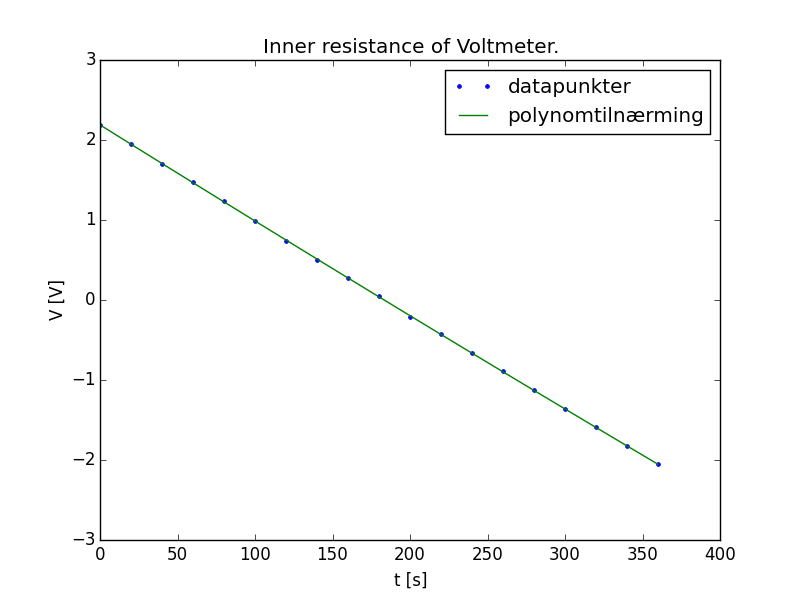
\includegraphics[width=400px]{\string~/Documents/3.Semester/FYS1120/Lab/GrunnleggjandeEMM/src/InnerRV.png}
      \caption{Me ser at målepunkta synker lineært for $\ln{U}$. Polynomtilnærminga stemmer bra med måleverdiane.}
    \end{figure}
    Programmet finner $\tau$ ved 
    \begin{align*}
      \tau = -\frac{\Delta{t}}{\Delta(\ln{U})}.
    \end{align*}
    Då finner me den indre resistansen ved 
    \begin{align*}
      \tau = RC.
    \end{align*}
    Programmet gjer oss utskrifta
    \begin{center}
      \input{\string~/Documents/3.Semester/FYS1120/Lab/GrunnleggjandeEMM/src/InnerRV.txt}
    \end{center}

  \subsection*{PRELAB-Oppgåve 1}
  \addcontentsline{toc}{subsection}{PRELAB-Oppgåve 1}
    Me nytter uttrykket for ladninga til ein kondensator som vert utlada. Denne finn me i boka og er gjeve ved
    \begin{align*}
      q = Q_0e^{-t/RC}.
    \end{align*}
    No setter me inn uttrykket for ladninga gjeve ved spenning og kapasitans.
    \begin{align*}
      C = \frac{Q}{V_{ab}} \qquad \Rightarrow \qquad Q = CV_{ab}.
    \end{align*}
    Då finner me for $V_0 = 2V_1$ at motstanden er gjeve ved
    \begin{align*}
      &CV_1 = CV_0e^{-t/RC} \qquad \Rightarrow \frac{1}{2}V_0 = V_0e^{-t/RC} \\
      &\Rightarrow \qquad \frac{1}{2} = e^{-t/RC} \qquad \Rightarrow \qquad \ln{\frac{1}{2}} = -\frac{t}{RC} \\
      &\Rightarrow \qquad \ln{1} - \ln{2} = -\frac{t}{RC} \qquad \Rightarrow \qquad \ln{2} = \frac{t}{RC} \\
      &\Rightarrow \qquad RC = \frac{t}{\ln{2}} \qquad \Rightarrow \qquad R = \frac{t}{C\ln{2}} \\
      &\Rightarrow \qquad R = \frac{20\text{ s}}{(1\times10^{-6}\text{ F})\ln{2}} \approx 29\text{ M}\Omega.
    \end{align*}

  \subsection*{Oppgåve 1.2}
  \addcontentsline{toc}{subsection}{Oppgåve 1.2}
    Når me lader opp kondensatoren så skjer dette motstandsfritt (med unntak av leidningar). Ved utladning tek det lengre tid då kondensatoren må gjennom voltmeteret som har ein 
    enorm indre resistans.




\newpage


\section*{Indre resistans i eit amperemeter}
\addcontentsline{toc}{section}{Indre resistans i eit amperemeter}


  \subsection*{Oppgåve 2.1}
  \addcontentsline{toc}{subsection}{Oppgåve 2.1}
    Me koplar resistansen og amperemeteret i serie og koplar voltmeteret i parallell med amperemeteret.
    Måleverdiane er gjeve ved
    \begin{center}
      \begin{tabular}{|l||l|l|}
        \hline
        $R$ [$\Omega$] & $I$ [A] & $V$ [V] \\
        \hline
        \input{\string~/Documents/3.Semester/FYS1120/Lab/GrunnleggjandeEMM/src/Oppgave2.1table.txt}
        \hline
      \end{tabular}
    \end{center}


  \subsection*{PRELAB-Oppgåve 2}
  \addcontentsline{toc}{subsection}{PRELAB-Oppgåve 2}
    Me nytter det same programmet me nytta i utrekningane våre av Hall-effekten.
    \verbatiminput{\string~/Documents/3.Semester/FYS1120/Lab/Hall-effekt/src/PRELABOppgave1.py}

  
  \subsection*{Oppgåve 2.2}
  \addcontentsline{toc}{subsection}{Oppgåve 2.2}
     Då får me ut målepunkta med polynomtilnærminga
    \begin{figure}[H]
      \centering
      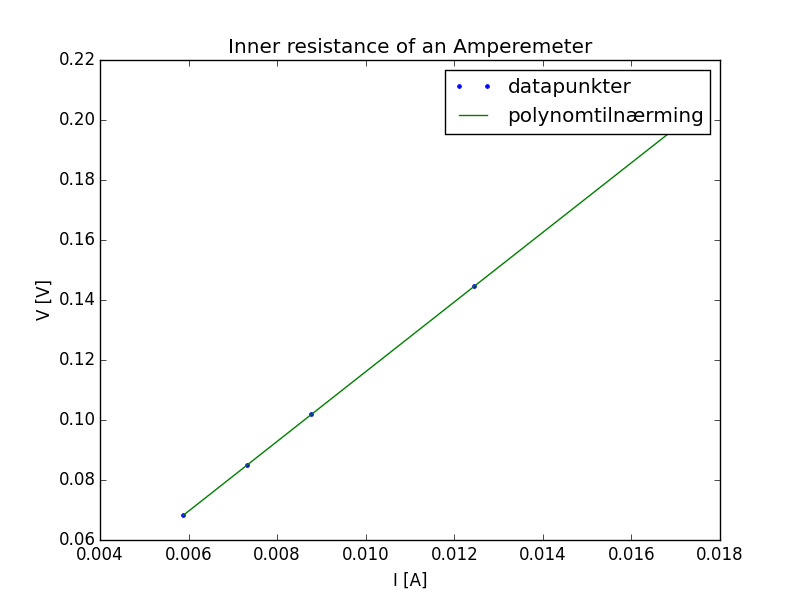
\includegraphics[width=400px]{\string~/Documents/3.Semester/FYS1120/Lab/GrunnleggjandeEMM/src/InnerRA.png}
      \caption{Me får ein ny lineær graf kor tilnærminga fylgjer tett.}
    \end{figure}

    Programmet $\texttt{Oppgave2.1.py}$ finner den indre resistansen ved
    \begin{align*}
      R = \frac{\Delta V}{\Delta I}.
    \end{align*}
    Me får utskrifta
    \begin{center}
      \input{\string~/Documents/3.Semester/FYS1120/Lab/GrunnleggjandeEMM/src/InnerRA.txt}
    \end{center}


\newpage


\section*{Indre resistans i eit termoelement (Peltier-element)}
\addcontentsline{toc}{section}{Indre resistans i eit termoelement (Peltier-element)}


  \subsection*{Oppgåve 3.1}
  \addcontentsline{toc}{subsection}{Oppgåve 3.1}
    Me kopla Peltier-elementet til voltmeteret og la ei hand over elementet. Me såg då at spenninga steig drastisk som ein følgje av temperaturtilførsel frå handa. Når me snudde 
    side på elementet vert spenninga negativ når me auka temperaturen. Ved kopling til ei straumkjelde merka me at elementet vart varmare på den eine sida og kaldare på den andre.


  \subsection*{Oppgåve 3.2}
  \addcontentsline{toc}{subsection}{Oppgåve 3.2}
    No nyttar me ein kopp med varmt vatn til å varme opp Peltier-elementet og koplar det til voltmeteret i serie med resistansen.
    Måleverdiane ser me i tabellen under.
    \begin{center}
      \begin{tabular}{|l|l|}
        \hline
        $R$ [$\Omega$] & $V$ [V] \\
        \hline
        \input{\string~/Documents/3.Semester/FYS1120/Lab/GrunnleggjandeEMM/src/Oppgave3.2table.txt}
        \hline
      \end{tabular}
    \end{center}



  \subsection*{Oppgåve 3.3}
  \addcontentsline{toc}{subsection}{Oppgåve 3.3}
    \begin{figure}[H]
      \centering
      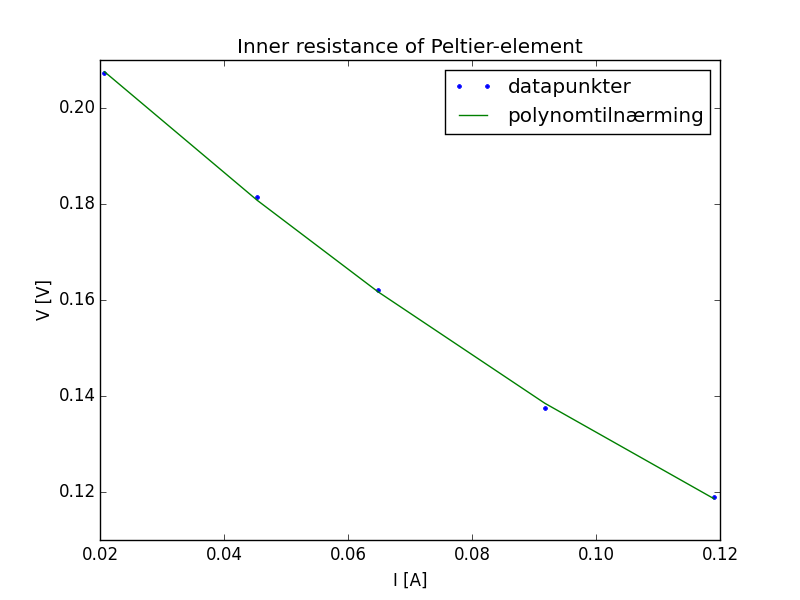
\includegraphics[width=400px]{\string~/Documents/3.Semester/FYS1120/Lab/GrunnleggjandeEMM/src/InnerRP.png}
      \caption{Me har ei ny lineær nedgang i potensialet som ein funksjon av straum.}
    \end{figure}

    Me forventa ei lineær nedgang. Programmet $\texttt{Oppgave3.2.py}$ gjer oss utskrifta
    \begin{center}
      \input{\string~/Documents/3.Semester/FYS1120/Lab/GrunnleggjandeEMM/src/InnerRP.txt}
    \end{center}
    Me fann $R_{i}$ ved formelen
    \begin{align*}
      R_i = -\frac{\Delta V}{\Delta I},
    \end{align*}
    kor minusteiknet kjem frå omforming av formelen
    \begin{align}
      U_{ab} = \varepsilon - R_iI.
    \end{align}
    Me fann $\varepsilon$ ved likning (1) for mange forskjellige verdiar og såg at han var konstant.





\newpage




\section*{Firepunktsmåling av resistans}
\addcontentsline{toc}{section}{Firepunktsmåling av resistans}


  \subsection*{Oppgåve 4.1}
  \addcontentsline{toc}{subsection}{Oppgåve 4.1}
    Me kopla amperemeteret og motstanden i serie. Fyrst brukte me ei firepunktsmåling kor voltmeteret gjekk gjennom motstanden og 
    deretter over. Me bytta mellom ein aluminiumsmotstand og ein kopparmotstand.
    Måleverdiar samt utrekna verdiar for motstand ved $R_4$ for firepunktsmåling og $R_2$ ved topunktsmåling. Fyrste tabell gjer oss for aluminium og den andre for koppar.
    \begin{center}
      \begin{tabular}{|l||l|l|||l||l|l|}
        \hline
        $R_4$ [$\Omega$] & $I_4$ [A] & $V_4$ [V] & $R_2$ [$\Omega$] & $I_2$ [A] & $V_2$ [V] \\
        \hline
        \input{\string~/Documents/3.Semester/FYS1120/Lab/GrunnleggjandeEMM/src/Oppgave4A.txt}
        \hline
      \end{tabular}
    \end{center}

    \begin{center}
      \begin{tabular}{|l||l|l|||l||l|l|}
        \hline
        $R_4$ [$\Omega$] & $I_4$ [A] & $V_4$ [V] & $R_2$ [$\Omega$] & $I_2$ [A] & $V_2$ [V] \\
        \hline
        \input{\string~/Documents/3.Semester/FYS1120/Lab/GrunnleggjandeEMM/src/Oppgave4C.txt}
        \hline
      \end{tabular}
    \end{center}

    Me ser at resistansane held seg tilnærma konstant uavhengig av straum. Differansen går som ein faktor $1.0\times10^{-2}$.

\newpage




\section*{Magnetfeltet til jordkloten}
\addcontentsline{toc}{section}{Magnetfeltet til jordkloten}


  \subsection*{PRELAB-Oppgåve 3}
  \addcontentsline{toc}{subsection}{PRELAB-Oppgåve 3}
    Me nyttar definisjonen av Faradays lov. Då kan me skrive
    \begin{align*}
      \varepsilon = -N\frac{d\Phi_{B}}{dt} = -\frac{d}{dt}\left( NBA\cos(\phi(t)) \right),
    \end{align*}
    kor $\phi(t) = \omega t$. Me deriverer med hensyn på tid og setter inn $\varepsilon = \varepsilon_0$. Det gjer oss
    \begin{align}
      &\varepsilon_0 = NBA\omega\sin(\omega t).
    \end{align}
    Me ser at forholdet mellom $\omega$ og $t_2 - t_1$ gjer oss vinkelen $\phi(t_2 - t_1)$. Då vil
    \begin{align*}
      \omega \propto \frac{1}{t_2 - t_1}.
    \end{align*}
    Frå likning (2) ser me at $\varepsilon_0$ vil ha sin største verdi når $\omega t = \frac{\pi}{2}$.



  \subsection*{Oppgåve 5.1}
  \addcontentsline{toc}{subsection}{Oppgåve 5.1}
    Me brukte eit kompass til å avgjere vinkelen mellom bakken og $B$-feltet til jorda. Deretter satte me spolen normalt på retninga til $B$-feltet. Me dreier spolen med ein 
    konstant vinkelhastighet $180$ grader.
    Me bruker målepunkta under.
    \begin{center}
      \begin{tabular}{|l|l|}
        \hline
        $t$ [s] & $\varepsilon_0$ [V] \\
        \hline
        \input{\string~/Documents/3.Semester/FYS1120/Lab/GrunnleggjandeEMM/src/Oppgave5table.txt}
        \hline
      \end{tabular}
    \end{center}
    Programmet $\texttt{Oppgave5.py}$ gjer oss gjennomsnittsverdien for $B$ ved å rekne  ut 
    \begin{align*}
      B = \frac{\varepsilon t}{4NA}.
    \end{align*}
    Denne formelen får me ved å sjå på grafen i oppgåveteksten og gjer ei tilnærming ved å behandle kurva som to trekantar.
    \begin{center}
      \input{\string~/Documents/3.Semester/FYS1120/Lab/GrunnleggjandeEMM/src/MeanValue.txt}
    \end{center}
    Dette er ei god tilnærming då magnetfeltet til jordkloten ligg mellom $25$ $\mu$T - $65$ $\mu$T.

    Me kan ikkje gje ei tilnærming av $B$ ved å ta gjennomsnittet av $\varepsilon_0$ og $t_2 - t_1$ separat då dei er avhengige av einannan.


\section*{Programma}
\addcontentsline{toc}{section}{Programma}
  \subsection*{Oppgave1.1.py}
  \addcontentsline{toc}{subsection}{Oppgave1.1.py}
    \verbatiminput{\string~/Documents/3.Semester/FYS1120/Lab/GrunnleggjandeEMM/src/Oppgave1.1.py}

  \subsection*{Oppgave2.1.py}
  \addcontentsline{toc}{subsection}{Oppgave2.1.py}
    \verbatiminput{\string~/Documents/3.Semester/FYS1120/Lab/GrunnleggjandeEMM/src/Oppgave2.1.py}


  \subsection*{Oppgave3.2.py}
  \addcontentsline{toc}{subsection}{Oppgave3.2.py}
    \verbatiminput{\string~/Documents/3.Semester/FYS1120/Lab/GrunnleggjandeEMM/src/Oppgave3.2.py}



  \subsection*{Oppgave4.py}
  \addcontentsline{toc}{subsection}{Oppgave4.py}
    \verbatiminput{\string~/Documents/3.Semester/FYS1120/Lab/GrunnleggjandeEMM/src/Oppgave4.py}


  \subsection*{Oppgave5.py}
  \addcontentsline{toc}{subsection}{Oppgave5.py}
    \verbatiminput{\string~/Documents/3.Semester/FYS1120/Lab/GrunnleggjandeEMM/src/Oppgave5.py}



\end{document}
